% Provenance (never printed): old seconde/premiere S material on water as a
% resource (stocks and flows of the water cycle, residence times, groundwater,
% overuse as a physical fact); see sources/book2/PROVENANCE.md. Residence
% times are computed in figdata/grade-10/residence_times.py, the Aral Sea
% budget in figdata/grade-10/aral_sea.py.
\chapter{淡水资源}\label{ch:g10:freshwater-resources}

1960 年，咸海位于中亚沙漠之中，是世界第四大湖泊。
两条大河由远方山区的冰雪与降雨补给，注入咸海，却没有河水流出。
1960 年代，这两条河的河水被引去灌溉沙漠。
卫星记录了随后发生的变化：湖泊已断裂成数片，
湖底大部分如今已成干地。造成这一切的原因，
绝不是气候变化，而是灌溉：每年流入湖中的水远少于湖面蒸发掉的水量。
本章统计地球上水的总量，说明水储存在何处、
流动有多快，并指出水资源首先是一种流动：当从储库中取走的水
多于流入的水时，储库就会排空，
排空的速率可由一个简单的收支模型预测。
% ledger: nasa:aral, gaybullaev:aral-1960, micklin:aral

\begin{omfigure}
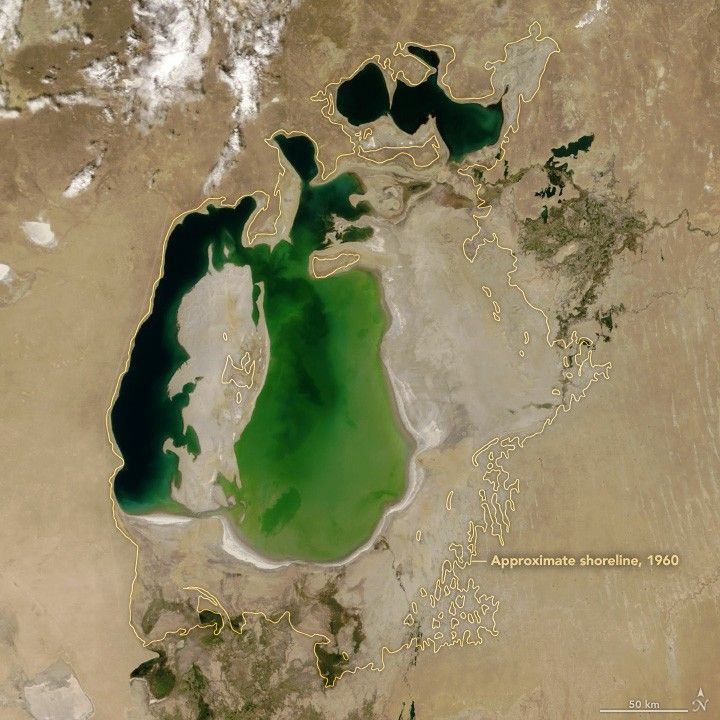
\includegraphics[width=0.47\linewidth]{images/book2/g10-nasa-aral-2000.jpg}\hspace{0.03\linewidth}%
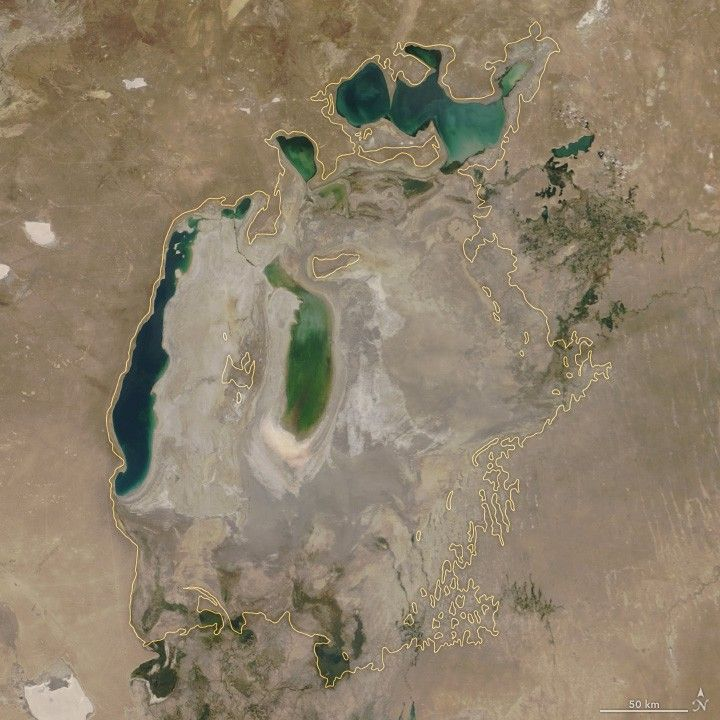
\includegraphics[width=0.47\linewidth]{images/book2/g10-nasa-aral-2018.jpg}

{\small 由 NASA Terra 卫星上 MODIS 仪器拍摄的咸海影像，
分别为 2000 年 8 月（左）和 2018 年 8 月（右）；黄线为 1960 年湖岸线的大致位置。
比例尺为 \qty{50}{km}。图像来源：NASA Earth
Observatory。}
\end{omfigure}

\begin{recall}
水循环使水在海洋、大气和陆地之间迁移：
蒸发、凝结成云、降水和径流；水的总质量
守恒（见物理各册）。具有连通孔隙的岩石是
透水的；地下水位以下，其孔隙充满水，
能持留并透过足够水量以供水井取用的岩层，即为
含水层（见第 1 册，六年级）。地球上的水大部分是
咸水（见第 1 册，二年级）。河流带走其\omterm{def:g10:drainage-basins:drainage-basin}{流域}内的水；
其\omterm{def:g10:drainage-basins:discharge}{流量}为每秒流过的水量（见\cref{ch:g10:drainage-basins}）。
\end{recall}

\section{水在何处}

地球约含有 13.9 亿立方千米的水，几乎全部
位于海洋中；仅 \qty{2.5}{\percent} 为淡水。而淡水中的大部分
难以利用：超过三分之二冻结在冰盖和冰川中，
其余近三分之一埋藏于地下。
% ledger: usgs:water-stocks

\begin{center}
\small
\begin{tabular}{|l|r|r|}
\hline
\textbf{储库} & \textbf{体积（\unit{km^3}）} & \textbf{占淡水的比例} \\ \hline
海洋、海和海湾 & \num{1338000000} & （咸水） \\ \hline
冰盖、冰川和永久积雪 & \num{24064000} & \qty{68.7}{\percent} \\ \hline
淡水地下水 & \num{10530000} & \qty{30.1}{\percent} \\ \hline
地下冰和永久冻土 & \num{300000} & \qty{0.86}{\percent} \\ \hline
淡水湖泊 & \num{91000} & \qty{0.26}{\percent} \\ \hline
土壤水分 & \num{16500} & \qty{0.05}{\percent} \\ \hline
大气 & \num{12900} & \qty{0.04}{\percent} \\ \hline
河流 & \num{2120} & \qty{0.006}{\percent} \\ \hline
\end{tabular}

{\small 世界水量的一种估计，据 Shiklomanov（1993）整理，
数据来自 U.S. Geological Survey。未计入咸水地下水（\num{12870000}~\unit{km^3}）
及咸水湖。}
\end{center}
% ledger: usgs:water-stocks

河流和淡水湖泊是人们用水的主要来源，
二者合计所含水量不足全部水量的万分之一。然而
河流几乎从不长期干涸：它们不是储存的水体，而是流动的水，
每场雨都会使其得到补充。

\section{储量与通量}

\begin{definition}[储量；通量]\label{def:g10:freshwater-resources:stock}
在水的收支中，\emph{储量}\index{储量（水）}是指
某一时刻储存于储库（海洋、大气、冰、含水层、湖泊等）中的水量，
可用体积或质量表示。\emph{通量}\index{通量（水）}是指
单位时间内从一个储库转移到另一个储库的水量，
例如以立方千米每年为单位。
\end{definition}

\omterm{def:g10:freshwater-resources:stock}{储量}只能通过\omterm{def:g10:freshwater-resources:stock}{通量}而改变：流入量减去流出量。当
两者相等时，\omterm{def:g10:freshwater-resources:stock}{储量}处于\emph{稳态}：其量保持不变，
尽管其中的水始终在被更新。

\begin{omfigure}
\begin{tikzpicture}[font=\footnotesize, >={Stealth[length=6pt]}]
  % ocean, land, atmosphere
  \fill[omSea] (0,0) rectangle (6.4,1.6);
  \fill[omLithAlluv] (6.4,0) -- (6.4,1.6) -- (8.2,2.1) -- (10.4,2.6) -- (12,2.9) -- (12,0) -- cycle;
  \fill[omLithSand!60] (6.4,0) -- (12,0) -- (12,1.0) -- (6.4,0.7) -- cycle;
  \draw[black!50] (6.4,1.6) -- (8.2,2.1) -- (10.4,2.6) -- (12,2.9);
  \fill[omIce] (10.6,2.65) -- (11.3,3.35) -- (12,2.9) -- cycle;
  \node[align=center] at (3.2,0.75) {\textbf{海洋}\\\num{1335040}};
  \node[align=center] at (9.3,1.35) {土壤水分 122\\湖泊和河流 178};
  \node[align=center] at (9.3,0.35) {地下水 \num{15300}};
  \node[align=center] at (11.2,2.25) {冰 \\\num{26350}};
  % atmosphere
  \draw[black!30, rounded corners=8pt, fill=omWxCloud] (1.0,4.6) rectangle (11.0,5.6);
  \node[align=center] at (6.0,5.1) {\textbf{大气} 12.7};
  % fluxes
  \draw[->, omProp, line width=1.4pt] (1.4,1.7) -- node[left, align=right] {蒸发 \\413} (1.4,4.5);
  \draw[->, omWxRain, line width=1.4pt] (4.4,4.5) -- node[pos=0.3, right, align=left] {降水 \\373} (4.4,1.7);
  \draw[->, omWxRain, line width=1.4pt] (7.6,4.5) -- node[pos=0.7, left, align=right] {降水 \\113} (7.6,2.05);
  \draw[->, omProp, line width=1.4pt] (10.0,2.6) -- node[right, align=left] {蒸发和 \\蒸腾 73} (10.0,4.5);
  \draw[->, black!60, line width=1.2pt] (4.9,5.85) -- node[above] {陆地上空输送的水蒸气：40} (7.4,5.85);
  \draw[->, omRiver, line width=1.4pt] (7.6,1.2) -- node[above, inner sep=2pt] {径流 40} (6.0,1.2);
\end{tikzpicture}

{\small 20 世纪 90 年代的全球水循环（示意图，未按比例绘制）。\omterm{def:g10:freshwater-resources:stock}{储量}
以千 \unit{km^3} 计，\omterm{def:g10:freshwater-resources:stock}{通量}以千 \unit{km^3} 每年计。
数据引自 Trenberth 等人（2007）。各\omterm{def:g10:freshwater-resources:stock}{储量}的估计值因研究而异，
请将此处的地下水和冰量与上表对照。}
\end{omfigure}
% ledger: trenberth:water-cycle

水循环是平衡的。每年海洋因蒸发损失 \num{413000}~\unit{km^3}，
并以雨雪形式回收 \num{373000}，另由
河流回收 \num{40000}。大气获得 $413\,000 + 73\,000 = \num{486000}$~\unit{km^3}，
并输出 $373\,000 + 113\,000$，两者相等。陆地接收降水
\num{113000}~\unit{km^3}，其中 \num{73000} 经
蒸发和植物叶片蒸腾返回大气，其余 \num{40000}
以河流和地下径流的形式流入海洋。
% ledger: trenberth:water-cycle

\begin{definition}[可再生淡水]\label{def:g10:freshwater-resources:renewable}
某地区的\emph{可再生淡水}\index{可再生淡水}是
每年由降水补给、流经该地区的淡水\omterm{def:g10:freshwater-resources:stock}{通量}，
以河流径流和地下水的形式流出。它是\omterm{def:g10:freshwater-resources:stock}{通量}，
以立方千米每年计，而非\omterm{def:g10:freshwater-resources:stock}{储量}。
\end{definition}

就全球陆地而言，每年抵达海洋的 \num{40000}~\unit{km^3} 即为
\omterm{def:g10:freshwater-resources:renewable}{可再生淡水}量。某地区可年复一年利用其可再生水，
而不致短缺。超出部分只能取自\omterm{def:g10:freshwater-resources:stock}{储量}，
\omterm{def:g10:freshwater-resources:stock}{储量}随之减少。

\section{停留时间}

一个水分子在储库中会停留多久？有的立即离开，
有的\omterm{def:g10:freshwater-resources:residence-time}{停留时间}则长得多；但平均而言，答案仅由\omterm{def:g10:freshwater-resources:stock}{储量}和
\omterm{def:g10:freshwater-resources:stock}{通量}决定。

\begin{definition}[停留时间]\label{def:g10:freshwater-resources:residence-time}
水在储库中的\emph{停留时间}\index{停留时间}是
水进入储库到离开储库之间平均经历的时间。
\end{definition}

\begin{proposition}[停留时间、储量与通量]\label{prop:g10:freshwater-resources:residence}
对于处于稳态的储库，\omterm{def:g10:freshwater-resources:stock}{储量}为 $S$，
并有\omterm{def:g10:freshwater-resources:stock}{通量} $F$ 流入与流出，则\omterm{def:g10:freshwater-resources:residence-time}{停留时间}为
\[
T = \frac{S}{F}.
\]
\end{proposition}

\begin{proof}
稳态下，每年有体积为 $F$ 的水进入，同时有体积为 $F$ 的水离开，
\omterm{def:g10:freshwater-resources:stock}{储量}保持为 $S$。经过时间 $S/F$ 后，已进入的水量为 $F \times S/F = S$，
与整个储库的容量相等。平均而言，开始时的水已被替换，
因此水在储库中的\omterm{def:g10:freshwater-resources:residence-time}{停留时间}为 $S/F$。
\end{proof}

\begin{example}[空气中的水]\label{ex:g10:freshwater-resources:atmosphere}
大气中储存的水为 \num{12700}~\unit{km^3}，
每年有 \num{486000}~\unit{km^3} 以雨雪形式降落。其
\omterm{def:g10:freshwater-resources:residence-time}{停留时间}为 $12\,700/486\,000 \approx \num{0.026}$ 年，
约 \num{9.5} 天：大气中的水每一两周就更新一次。一朵云
今天正在下雨的云，由几天前离开海洋或
地面的水组成。
\end{example}
% ledger: trenberth:water-cycle (t_atmosphere_days 9.5 in figdata/grade-10/residence_times.py)

同样的计算表明，河道中的水约需 \num{19} 天更新（
储水 $2120$~\unit{km^3}，每年输送 \num{40000}~\unit{km^3}）。湖泊与河流合计约需数年，
海洋约需 \num{3200} 年（
$1\,335\,040/413$ 千~\unit{km^3}）。地下水可能更慢：
某些含水层最深处的水已有数十万年之久。
% ledger: trenberth:water-cycle, usgs:water-stocks, sturchio:nubian-age

\begin{omfigure}
\begin{tikzpicture}
\begin{axis}[omrecord, xbar, xmode=log, log origin=infty, width=0.74\linewidth, height=5.6cm,
  xmin=1, xmax=1e9, ymin=-0.6, ymax=4.6, bar width=11pt,
  ytick={0,1,2,3,4}, yticklabels={大气, 河流, {湖泊和河流}, 海洋, {深层地下水（年龄）}},
  xtick={1,30.44,365.25,36525,3652500,365250000}, xticklabels={1 天, 1 个月, 1 年, 100 年, \num{10000} 年, 100 万年},
  xticklabel style={font=\scriptsize, rotate=25, anchor=north east}, yticklabel style={font=\small},
  xlabel={停留时间（对数刻度）}, label style={font=\small}, xmajorgrids]
\addplot[fill=omDef!45, draw=omDef!80!black] table[x=days, y=idx] {figdata/out/grade-10-residence_times-times.dat};
\draw[fill=omProp!45, draw=omProp!80!black] (axis cs:73050000,3.75) rectangle (axis cs:365250000,4.25);
\node[anchor=west, font=\scriptsize] at (axis cs:9.5,0) {\num{9.5} 天};
\node[anchor=west, font=\scriptsize] at (axis cs:19.4,1) {\num{19} 天};
\node[anchor=west, font=\scriptsize] at (axis cs:1625,2) {\num{4.5} 年};
\node[anchor=west, font=\scriptsize] at (axis cs:1180690,3) {\num{3200} 年};
\node[anchor=east, font=\scriptsize] at (axis cs:73050000,4) {\num{200000} 至 100 万年};
\end{axis}
\end{tikzpicture}

{\small 水的\omterm{def:g10:freshwater-resources:residence-time}{停留时间}由全球水循环的\omterm{def:g10:freshwater-resources:stock}{储量}除以\omterm{def:g10:freshwater-resources:stock}{通量}算得（蓝色），
以及撒哈拉东部地下深层水的实测年龄（橙色）。
对数坐标轴：从一年起，每个刻度间隔为前一刻度的百倍。数据来源：
Trenberth 等人（2007）；美国地质调查局；Sturchio 等人
（2004）。}
\end{omfigure}
% values computed in figdata/grade-10/residence_times.py

\omterm{def:g10:freshwater-resources:residence-time}{停留时间}反映储库恢复的快慢。从河流中取出的水，
几天便能被替换；受污染或被抽干的湖泊需要数年；积累
用了数千年的地下水，以人的一生为尺度来看，
根本得不到更新。

\begin{method}[水量收支]\label{met:g10:freshwater-resources:budget}
\begin{enumerate}
  \item 选定储库：湖泊、含水层、\omterm{def:g10:drainage-basins:drainage-basin}{流域}或大气。
  \item 列出流入和流出该储库的每一项\omterm{def:g10:freshwater-resources:stock}{通量}（流入：河流、降雨、渗漏；
        流出：河流、蒸发、抽水），并使用相同单位。
  \item 每年\omterm{def:g10:freshwater-resources:stock}{储量}的变化等于输入量之和减去
        输出量之和。
  \item 若\omterm{def:g10:freshwater-resources:stock}{储量}不变，则输入量等于输出量，\omterm{def:g10:freshwater-resources:residence-time}{停留时间}
        等于\omterm{def:g10:freshwater-resources:stock}{储量}除以二者中的任一个。
\end{enumerate}
\end{method}

\section{含水层作为储库}

渗入地面并到达地下水位的雨水会\emph{补给}
其下方的含水层。水随后缓慢穿过岩石的孔隙，
流向泉、河流或海。当透水层
倾伏于不透水层（如黏土）之下时，该层中的水处于
\emph{承压}状态：仅在该层出露于地表处获得补给，
而该处可能很远。

\begin{omfigure}
\begin{tikzpicture}[font=\footnotesize, >={Stealth[length=5pt]}]
  % layers dipping to the right
  \fill[lith shale] (0,0) -- (12,0) -- (12,0.8) -- (0,2.4) -- cycle;
  \fill[lith sandstone] (0,2.4) -- (12,0.8) -- (12,2.2) -- (2.2,3.5) -- (0,3.8) -- cycle;
  \fill[lith shale] (2.2,3.5) -- (12,2.2) -- (12,3.4) -- (3.6,3.9) -- cycle;
  % ground surface
  \draw[line width=0.8pt, brown!60!black] (0,3.8) -- (1.2,4.0) -- (2.2,3.9) -- (3.6,3.9) -- (6,3.6) -- (9,3.5) -- (12,3.4);
  \fill[omLithAlluv] (0,3.8) -- (1.2,4.0) -- (2.2,3.9) -- (2.2,3.5) -- (0,3.8) -- cycle;
  \fill[omLithAlluv] (2.2,3.9) -- (3.6,3.9) -- (2.2,3.5) -- cycle;
  \fill[omLithAlluv] (3.6,3.9) -- (6,3.6) -- (9,3.5) -- (12,3.4) -- (3.6,3.9) -- cycle;
  % water table in the unconfined part
  \draw[omDef, line width=1pt, dashed] (0,3.3) .. controls (1.0,3.35) and (1.8,3.2) .. (2.6,3.45);
  \node[anchor=south west, text=omDef, fill=white, fill opacity=0.8, text opacity=1, inner sep=1pt] at (0.05,2.75) {地下水位};
  % rain and recharge
  \foreach \x in {0.35,0.65,0.95,1.25} \draw[omWxRain, thick] (\x,4.9) -- (\x-0.15,4.4);
  \node[anchor=south, text=omWxRain] at (0.7,4.95) {降雨：补给};
  % flow arrows in the aquifer
  \draw[->, omDef, line width=1.1pt] (2.0,2.85) -- (4.4,2.55);
  \draw[->, omDef, line width=1.1pt] (5.4,2.4) -- (7.8,2.1);
  \draw[->, omDef, line width=1.1pt] (8.8,1.95) -- (11.2,1.65);
  % wells
  \draw[black!70, line width=1.6pt] (1.95,3.95) -- (1.95,2.9);
  \node[anchor=south] at (1.95,4.0) {水井};
  \draw[black!70, line width=1.6pt] (7.0,3.55) -- (7.0,1.9);
  \node[anchor=south] at (7.0,3.6) {水井};
  % labels
  \node[align=center, fill=white, fill opacity=0.85, text opacity=1, inner sep=1.5pt] at (1.5,0.8) {不透水黏土};
  \node[align=center, fill=white, fill opacity=0.85, text opacity=1, inner sep=1.5pt] at (8.6,2.95) {不透水黏土};
  \node[anchor=north, align=center] at (1.6,-0.1) {潜水含水层：\\补给区};
  \node[anchor=north, align=center] at (6.4,-0.1) {承压含水层};
  \node[anchor=north, align=center] at (10.6,-0.1) {古老的水，远离 \\补给区};
\end{tikzpicture}

{\small 透水砂岩中的一个含水层（示意）。雨水在其出露于地表处补给该含水层；
此处的地下水位可自由升降。
再往远处，黏土之下的含水层处于承压状态，其水
沿岩层缓慢流动：距补给区越远，
水就越古老。}
\end{omfigure}

\begin{definition}[化石地下水]\label{def:g10:freshwater-resources:fossil-groundwater}
\emph{化石地下水}\index{化石地下水}是指
很久以前进入含水层、常形成于较湿润气候时期，并且
当今补给在人类寿命尺度内无法使其更新的地下水。
\end{definition}

撒哈拉沙漠东部地下蕴藏着一个巨大的砂岩含水层。其最深处的水，
用一种稀有放射性氪同位素的衰变测定，其年龄为
\num{200000}至100万年。它缓慢地从埃及西南部的补给区流入，
其化学特征表明，它是在冰期的湿润时段以降雨形式落下的，
那时大西洋的湿润空气曾抵达该地区。
如今抽取的此类水属于正在被开采的\omterm{def:g10:freshwater-resources:stock}{储量}，而非\omterm{def:g10:drainage-basins:discharge}{流量}。
% ledger: sturchio:nubian-age

抽水量超过补给量时，地下水位下降。在美国中部的高平原
地区，含水层面积约 \num{175000} 平方英里
（\qty{453000}{km^2}）自约1950年起被抽取用于灌溉。至2015年，
其水位平均下降 \qty{4.8}{m}，部分地区最多达
\qty{71}{m}（234 英尺）；部分水井处
含水层约失去 2.73 亿英亩英尺的水，约 \qty{340}{km^3}。
% ledger: mcguire:high-plains (1 acre-foot = 1233.5 m3)

\begin{omfigure}
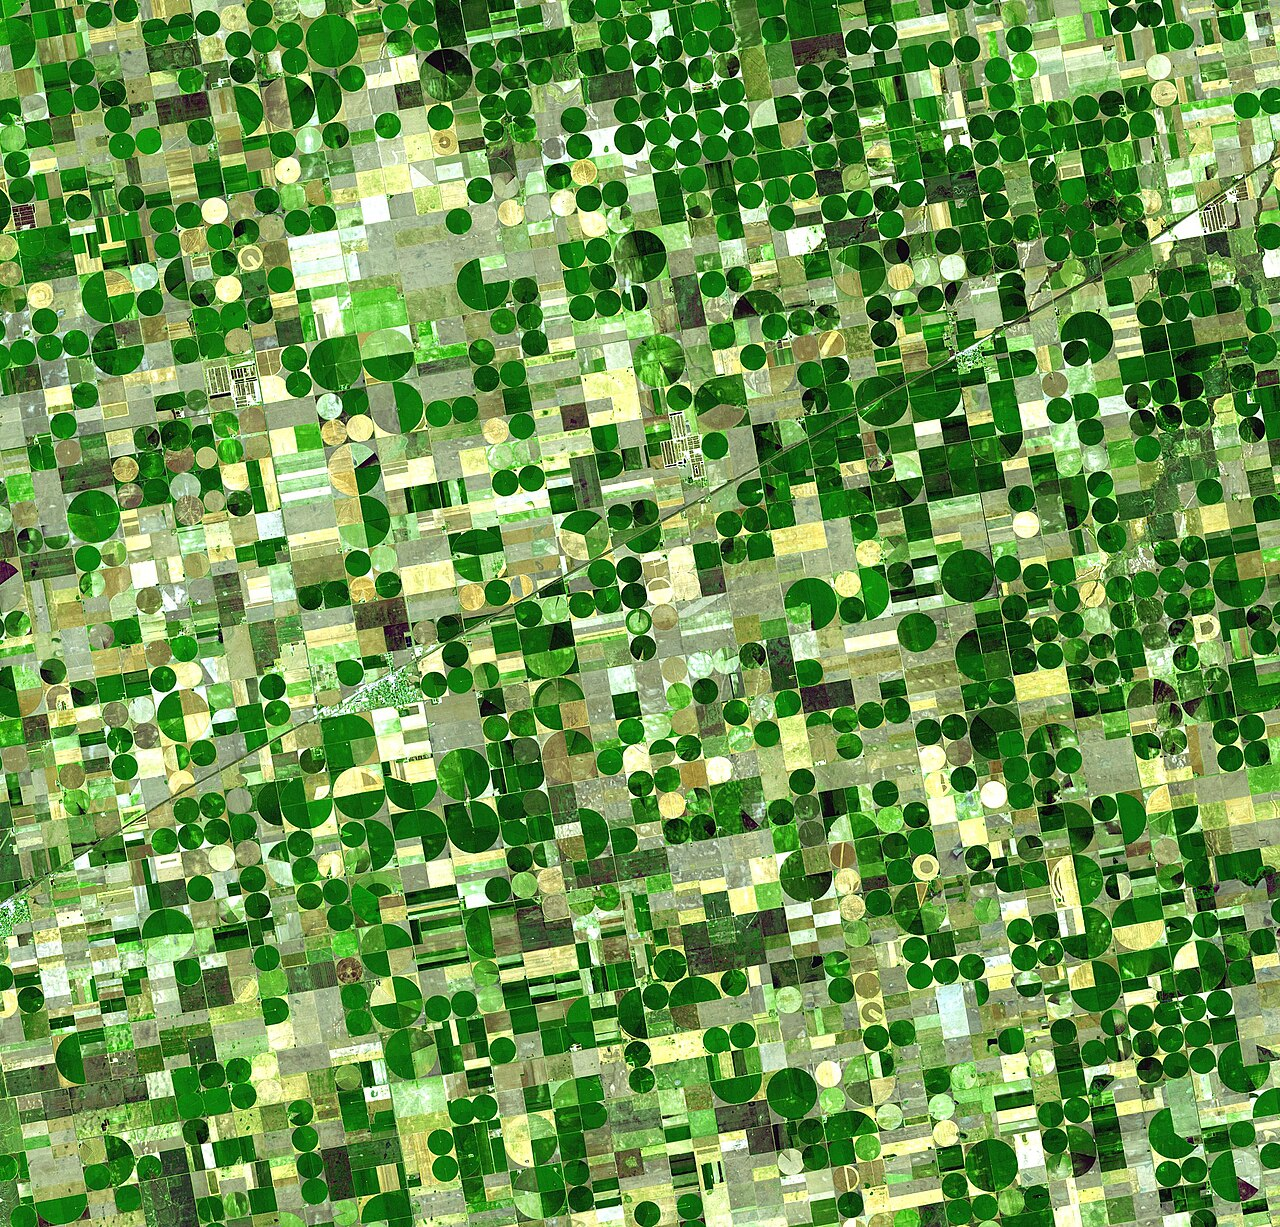
\includegraphics[width=0.5\linewidth]{images/book2/g10-nasa-kansas-center-pivot.jpg}

{\small 堪萨斯州萨布莱特附近的灌溉农田，由 NASA Terra 卫星上的 ASTER 仪器于
2001 年 6 月拍摄（约 \qty{37}{km} 宽）。每个圆形是一块农田，
由一根绕其中心转动的长喷灌臂浇灌；各圆形
直径为 \num{800} 和 \qty{1600}{m}。图像：NASA（公有领域）。}
\end{omfigure}

地下水无法从太空看到，但可以称量：两颗卫星
前后飞行，能感受到地球拉力的微小变化，该变化
由其下方来去的水的质量引起，并绘出陆地水\omterm{def:g10:freshwater-resources:stock}{储量}
在何处逐月升降。

\begin{omfigure}
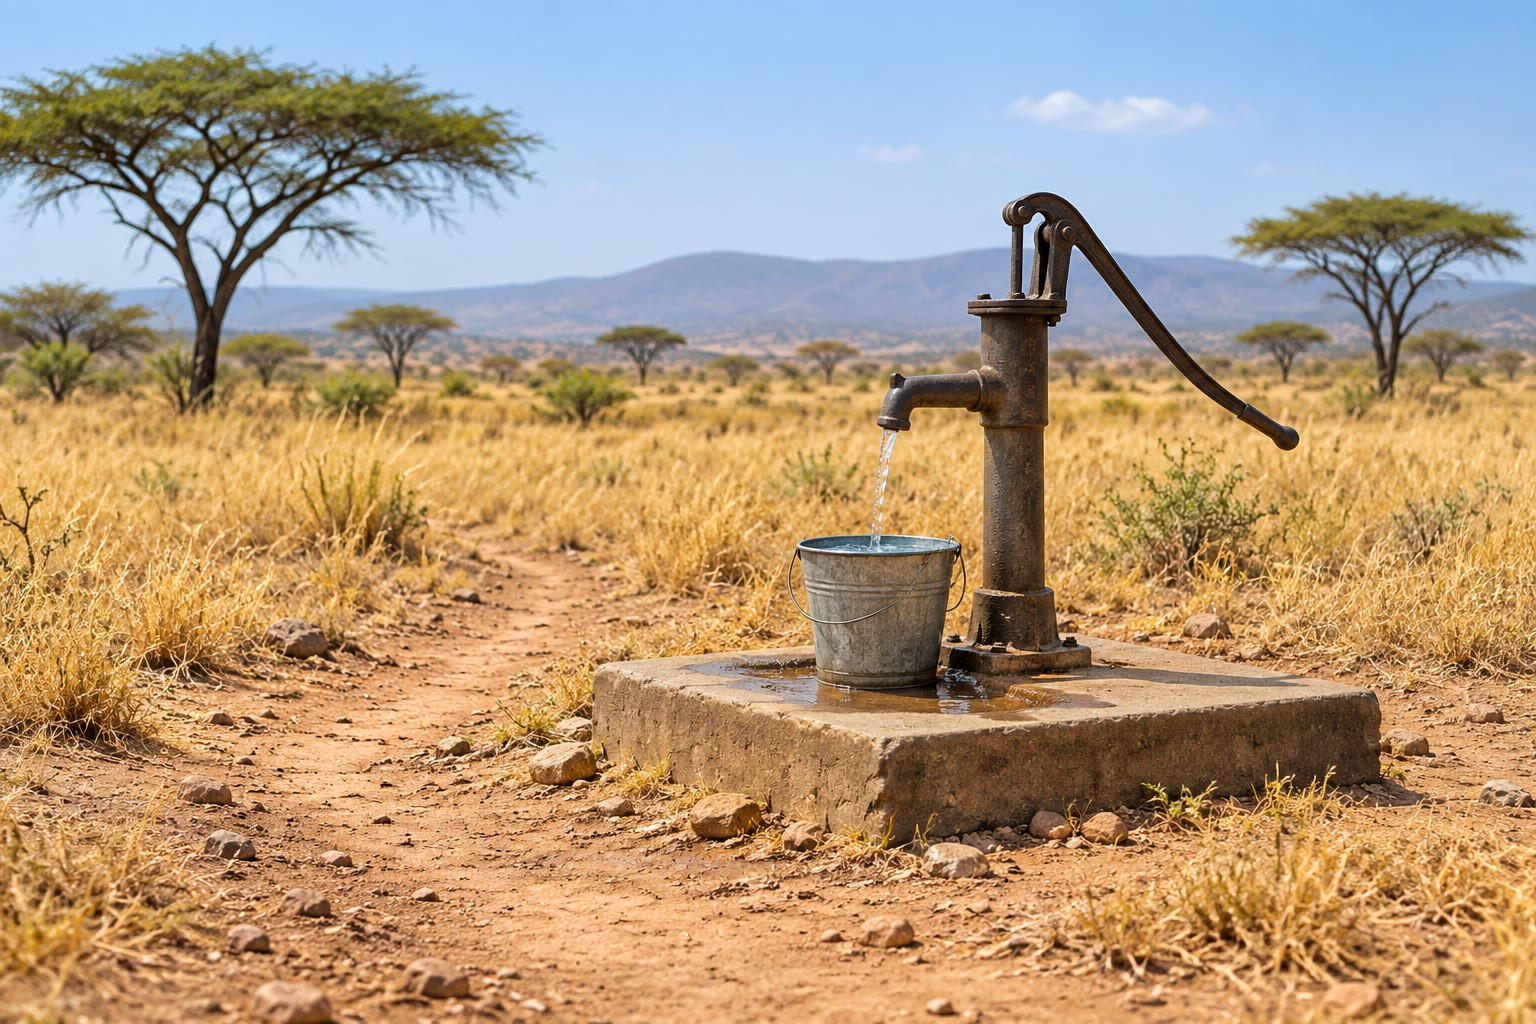
\includegraphics[width=0.55\linewidth]{images/book2/ai/g10-hand-pump-well.jpg}

{\small 干旱景观中一口水井上的手动泵：此处抽取的水
来自地下，不受旱季影响。}
\end{omfigure}

\section{作为物理事实的过度利用}

咸海没有出口：其两条河流阿姆河和
锡尔河的水仅通过蒸发离开。1960 年时，咸海面积为
\qty{68000}{km^2}，蓄水量 \qty{1093}{km^3}，其水中含盐 \qty{10}{g} 
每升。当年蒸发量为 \qty{71.1}{km^3}，湖面降雨
带来 \qty{9.4}{km^3}：要维持水位，湖泊每年需要
$71.1 - 9.4 = \qty{61.7}{km^3}$ 每年由其河流补入。
% ledger: gaybullaev:aral-1960, gaybullaev:aral-table

自 1960 年代起，河水被引向沙漠灌溉，几乎
没有任何河水流入湖中：1970 年代和 1980 年代，
每年常不足 \qty{2}{km^3}。蒸发仍在继续，湖泊
开始萎缩。其水量收支决定萎缩的速度。蒸发带走一层水，
其厚度取决于气候，此处每年约 1 米
（$71.1/68\,000 \approx \qty{0.00105}{km}$）。若入流停止，水位
每年约下降这一数值（扣除降雨）。湖泊萎缩时，其
面积随之缩小，蒸发量也随之减少，下降速度减慢；但
直到入流与蒸发重新达到平衡，水位才会停止下降。
% ledger: gaybullaev:aral-table (values computed in figdata/grade-10/aral_sea.py)

\begin{omfigure}
\begin{tikzpicture}
\begin{axis}[omrecord, name=vol, width=0.46\linewidth, height=5.4cm, xmin=1955, xmax=2012, ymin=0, ymax=1200,
  xtick={1960,1980,2000}, xticklabel style={/pgf/number format/1000 sep={}}, scaled y ticks=false,
  ylabel={体积 (\unit{km^3})}, xlabel={年}, tick label style={font=\small}, label style={font=\small},
  title={\small 水的体积}]
\addplot[omDef, line width=1pt, mark=*, mark size=1.3pt] table[x=year, y=volume] {figdata/out/grade-10-aral_sea-record.dat};
\end{axis}
\begin{axis}[omrecord, at={(vol.east)}, anchor=west, xshift=1.4cm, width=0.46\linewidth, height=5.4cm,
  xmin=1955, xmax=2012, ymin=0, ymax=140, xtick={1960,1980,2000},
  xticklabel style={/pgf/number format/1000 sep={}},
  ylabel={盐度 (\unit{g/L})}, xlabel={年}, tick label style={font=\small}, label style={font=\small},
  title={\small 盐度}]
\addplot[omProp, line width=1pt, mark=*, mark size=1.3pt] table[x=year, y=salinity] {figdata/out/grade-10-aral_sea-record.dat};
\end{axis}
\end{tikzpicture}

{\small 咸海 1960 至 2010 年：其水的体积降至
原来的十分之一，而蒸发遗留的盐分
则浓缩至原来的十三倍。数据来源：Gaybullaev 等（2012）。}
\end{omfigure}
% ledger: gaybullaev:aral-table

到 2010 年，湖水仅余 \qty{98}{km^3}，为 1960 年水体积的十分之一，覆盖面积达
\qty{14280}{km^2}；其盐度已达 \qty{130}{g/L}，
远高于海洋。湖面水位已下降超过 \qty{20}{m}。含盐的尘埃
从干涸的湖床上被风吹起。原因并不隐晦：湖泊的入流被切断，
而蒸发却未减少。
% ledger: gaybullaev:aral-table, gaybullaev:aral-1960, micklin:aral, nasa:aral

\section{练习}

\begin{exercise}[$\star$]\label{exo:g10:freshwater-resources:1}
定义\omterm{def:g10:freshwater-resources:stock}{储量}、\omterm{def:g10:freshwater-resources:stock}{通量}和\omterm{def:g10:freshwater-resources:residence-time}{停留时间}，并写出各自的单位。
\end{exercise}

\begin{exercise}[$\star$]\label{exo:g10:freshwater-resources:2}
根据世界水量表：全部水中淡水所占的比例是多少？在淡水中，
冰冻水与地下水各占多少比例？哪个储库
的水量最少？
\end{exercise}

\begin{exercise}[$\star$]\label{exo:g10:freshwater-resources:3}
定义\omterm{def:g10:freshwater-resources:renewable}{可再生淡水}与\omterm{def:g10:freshwater-resources:fossil-groundwater}{化石地下水}。为什么前者是\omterm{def:g10:freshwater-resources:stock}{通量}，
而后者是\omterm{def:g10:freshwater-resources:stock}{储量}？
\end{exercise}

\begin{exercise}[$\star$]\label{exo:g10:freshwater-resources:4}
世界淡水湖泊（\num{91000}~\unit{km^3}）的水量
是河流（\num{2120}~\unit{km^3}）的多少倍？
\end{exercise}

\begin{exercise}[$\star$]\label{exo:g10:freshwater-resources:5}
由\omterm{def:g10:freshwater-resources:residence-time}{停留时间}图可知，哪个储库的水更新最快，
哪个最慢？水在海洋中的\omterm{def:g10:freshwater-resources:residence-time}{停留时间}
是在大气中的多少倍？
\end{exercise}

\begin{exercise}[$\star\star$]\label{exo:g10:freshwater-resources:6}
大气中含水 \num{12700}~\unit{km^3}。
由每年进入大气的蒸发量（来自海洋的 \num{413000}，
来自陆地的 \num{73000}~\unit{km^3}）计算其\omterm{def:g10:freshwater-resources:residence-time}{停留时间}，
并与由离开大气的降水量算得的\omterm{def:g10:freshwater-resources:residence-time}{停留时间}相核对。
\end{exercise}

\begin{exercise}[$\star\star$]\label{exo:g10:freshwater-resources:7}
海洋含水 \num{1335040} 千~\unit{km^3}，
每年因蒸发损失 \num{413} 千~\unit{km^3}。计算其\omterm{def:g10:freshwater-resources:residence-time}{停留时间}。
若用进入海洋的水量计算，结果为何相同？
\end{exercise}

\begin{exercise}[$\star\star$]\label{exo:g10:freshwater-resources:8}
利用全球水循环的\omterm{def:g10:freshwater-resources:stock}{通量}，写出陆地的水量收支：陆地上降下多少水，
有多少返回大气，有多少形成径流。落在陆地上的降水中，
有多大比例返回大气？
\end{exercise}

\begin{exercise}[$\star\star$]\label{exo:g10:freshwater-resources:9}
高平原含水层在约 1950 至 2015 年间失去了约 2.732 亿英亩·英尺的水
（\num{1}~英亩·英尺 = \qty{1233.5}{m^3}）。将这一水量
换算为 \unit{km^3}，并与 1987 年咸海的水量
（\qty{345.6}{km^3}）进行比较。
\end{exercise}

\begin{exercise}[$\star\star$]\label{exo:g10:freshwater-resources:10}
高平原含水层的平均水位在约 1950 至 2015 年间下降了 \num{15.8} 英尺
（\num{1}~英尺 = \qty{0.3048}{m}）。这相当于多少米？
平均每年下降多少厘米？
\end{exercise}

\begin{exercise}[$\star\star$]\label{exo:g10:freshwater-resources:11}
某含水层储水 \qty{2}{km^3}，每年得到
\qty{0.01}{km^3} 的补给。求其水的\omterm{def:g10:freshwater-resources:residence-time}{停留时间}。现在水井每年
从中抽取 \qty{0.05}{km^3}。假设补给持续进行，且水井
是水离开含水层的唯一途径，
这些水能维持多久？
\end{exercise}

\begin{exercise}[$\star\star\star$]\label{exo:g10:freshwater-resources:12}
计算咸海 1960 年水的\omterm{def:g10:freshwater-resources:residence-time}{停留时间}
（水量 \qty{1093}{km^3}，每年蒸发 \qty{71.1}{km^3}）和 2010 年
（水量 \qty{98.1}{km^3}，每年蒸发 \qty{11.4}{km^3}）的
\omterm{def:g10:freshwater-resources:residence-time}{停留时间}。其蒸发量为何减少？
\end{exercise}

\begin{exercise}[$\star\star\star$]\label{exo:g10:freshwater-resources:13}
一个无出口的湖泊覆盖面积 \qty{100}{km^2}。蒸发每年从湖面带走
\qty{1.2}{m} 的水，降雨每年补充 \qty{0.2}{m}。
\begin{enumerate}
  \item 每年需要多少 \unit{km^3} 的入流，才能使水位保持稳定？
  \item 入流减半。第一年水位
        下降多少？
  \item 为什么在之后几年中下降速度会减慢？
\end{enumerate}
\end{exercise}

\begin{exercise}[$\star\star\star$]\label{exo:g10:freshwater-resources:14}
在沙漠中，降雨每年以 \qty{1}{mm} 的水量补给含水层，
含水层厚 \qty{100}{m}，水充满其 \qty{20}{\percent} 的
体积。补给充满它需要多长时间？并与
撒哈拉含水层深层水的年龄作比较。
\end{exercise}

\begin{exercise}[$\star\star\star$]\label{exo:g10:freshwater-resources:15}
高平原含水层面积约 \qty{453000}{km^2}，截至 2015 年
已损失约 \qty{337}{km^3} 的水。若将这些水均匀铺在
整个含水层上，相当于多厚的水层？其水位平均下降了 \qty{4.8}{m}。
为什么水位下降幅度大于所损失的水层厚度？
\end{exercise}

\section{问题：咸海的水量收支}

\begin{problem}[{周末问题——湖泊会以多快的速度消失？}]
\label{pb:g10:freshwater-resources:1}
% ledger: gaybullaev:aral-table, gaybullaev:aral-1960, micklin:aral (values computed in figdata/grade-10/aral_sea.py)
下表给出咸海四个年份的水量收支（体积以
\unit{km^3}，盐度以每升所含盐的克数表示）。1960 年，该湖覆盖面积为
\qty{68000}{km^2}。
\begin{center}
\small
\begin{tabular}{|c|c|c|c|c|c|}
\hline
年份 & 河流入\omterm{def:g10:drainage-basins:discharge}{流量} & 湖面降雨 & 蒸发量 & 体积 & 盐度 \\ \hline
1960 & 42.0 & 9.4 & 71.1 & 1093.0 & 10.0 \\ \hline
1984 & 0.3 & 3.5 & 47.9 & 502.7 & 21.9 \\ \hline
1987 & 1.0 & 6.2 & 36.8 & 345.6 & 25.0 \\ \hline
1989 & 3.1 & 5.3 & 35.3 & 327.2 & 30.0 \\ \hline
\end{tabular}

{\small 数据来源：Gaybullaev 等（2012）。}
\end{center}

\medskip
\noindent\textbf{第一部分——1960 年的湖泊。}
\begin{enumerate}
  \item 1960 年该湖的平均深度是多少？
  \item 用立方米表示其体积。
  \item 该湖所含盐的质量为多少吨？
  \item 若只考虑蒸发这一输出途径，其水的\omterm{def:g10:freshwater-resources:residence-time}{停留时间}是多少？
  \item 为什么无出口的湖泊只能通过蒸发（以及
        渗漏）失水？
\end{enumerate}

\medskip
\noindent\textbf{第二部分——湖泊的需水量。}
\begin{enumerate}[resume]
  \item 蒸发使湖泊在
        1960 年失去的水层厚度（以米计）是多少？
  \item 降雨增加的水层厚度是多少？
  \item 河流入\omterm{def:g10:drainage-basins:discharge}{流量}为多少时，恰好能与蒸发和降雨相平衡？
  \item 两条河流每年平均从山区带来约 \qty{79}{km^3} 和
        \qty{37}{km^3} 的水量。这些水中有多大比例，
        是湖泊所需？
\end{enumerate}

\medskip
\noindent\textbf{第三部分——1980 年代后期的湖泊。}
\begin{enumerate}[resume]
  \item 写出 1987 年的水量收支：输入、输出和净变化。
  \item 1984 年至 1989 年间，体积从 \qty{502.7}{km^3} 降至
        \qty{327.2}{km^3}。平均每年下降多少？与
        1987 年的收支作比较。
  \item 假设每平方千米湖面的蒸发失水量，
        与 1960 年相同。1987 年该湖的面积是多少？
  \item 这相当于其 1960 年面积的多大比例？
  \item 蒸发量为何从 \qty{71.1}{km^3} 降至
        \qty{36.8}{km^3}？
  \item 1987 年，湖泊仍保有其 1960 年体积的多大比例？
\end{enumerate}

\medskip
\noindent\textbf{第四部分——盐分与水位。}
\begin{enumerate}[resume]
  \item 若 1960 年的全部盐分都保留在水中，1987 年的
        盐度应为多少？
  \item 表中给出的盐度为 \qty{25.0}{g/L}。两者之差说明了什么？
  \item 若既无入流也无降雨，
        水位每年将下降多少？
  \item 1987 年，河流和降雨共增加了多厚的水层，
        （按第 12 题的面积折算）？
  \item 1987 年咸海水位下降了多少？
\end{enumerate}
\end{problem}
